
%\documentclass[paper]{geophysics}
\documentclass[manuscript,revised]{geophysics}
\usepackage{amsmath,amssymb}
\usepackage[english, ruled]{algorithm2e}

% An example of defining macros
\newcommand{\rs}[1]{\mathstrut\mbox{\scriptsize\rm #1}}
\newcommand{\rr}[1]{\mbox{\rm #1}}

\begin{document}
\title{Estimating total magnetization direction using equivalent-layer technique}

\renewcommand{\thefootnote}{\fnsymbol{footnote}} 

\ms{GEO-2019XXXX} % manuscript number

\address{
\footnotemark[2] Observat\'orio Nacional, Rio de Janeiro, Brazil\\
\footnotemark[1] Corresponding author: reisandreluis@gmail.com}
\author{Andr\'e L. A. Reis\footnotemark[2] \footnotemark[1], Vanderlei C. Oliveira Jr.\footnotemark[2] and  Val\'eria C. F. Barbosa \footnotemark[2]}

\footer{Example}
\lefthead{Reis, A.L.A. \& Oliveira Jr, V.C. \& Barbosa, V. C. F.}
\righthead{Determining total magnetization direction}

\maketitle


% % The body text
\begin{abstract}
We developed a new method for estimating the total magnetization direction of magnetic sources based on equivalent-layer technique using total-field anomaly data. This approach does not impose strong information either about the shape or about the depth of the sources, and does not require a regularly spaced data. Usually, the equivalent-layer technique is used for processing total-field anomaly data by estimating a 2D magnetic-moment distribution over a fictitional layer composed by dipoles below the observation plane. When the magnetization direction of equivalent sources is almost the same as the true body, the estimated magnetic property over the layer is all positive. Iteratively, the proposed method imposes zeroth-order Tikhonov regularization and positivity constraint on the estimated magnetic moment over the layer and estimate the magnetization direction of the geological sources. Mathematically, the algorithm solves least-squares problems in two steps: the first one solves a linear inverse problem for estimating a 2D magnetic-moment distribution within the equivalent layer and the second solves a nonlinear inverse problem for magnetization direction of the magnetized sources. We test the methodology by applying to synthetic data for different geological scenarios, and the results show that the method can be a powerful tool for estimating the magnetization direction of a set of bodies. Tests on field data from Goias Alkaline Province (GAP), center of Brazil, over Montes Claros complex suggests intrusions with remarkable strong remanent magnetization, in agreement with the current literature for this region. 
\end{abstract}
%\section{Introduction}

%% The importance of magnetization direction and techniques
Most of  magnetic methods require knowledge of the magnetization direction, otherwise 
they yield unsatisfactory interpretations of the exploration targets. This fact has 
been propelled the development of several techniques for estimating magnetization 
direction over the last 50 years. The strategies for estimating this quantity can be 
divided into two main groups. The first one comprises the methods which presume a prior 
information about the shape of geological sources. The iterative method presented by 
\cite{bhattacharyya1966} presumed that the magnetic source has a rectangular prismatic shape. 
\cite{emilia_massey_1974} approximated a seamount by a set of stacked 
prisms with uniform magnetization direction and variable magnetization intensity. 
\cite{parker_etal_1987} approximated the geometry of a seamount by using a 
covering of triangular facets and estimate the internal magnetization closest to 
a uniform solution.
\cite{medeiros_silva_1995} presented a method that estimates the total magnetization 
direction and the spatial orientation of an isolated source having three othogonal planes of 
symmetry. 
\cite{kubota2005} also approximated a seamount by a set of juxtaposed prisms, but estimate a 
magnetization direction for each one. 
Finally, \cite{oliveirajr_etal_2015} approximated the magnetic sources by spherical bodies with 
known centers for estimating their magnetization directions. 
The second group is formed by methods which do not presume any information about the shape of the 
magnetic sources. \cite{fedi_etal_1994}, for example, proposed a method that determines the best 
magnetization direction among a set a tentative values used to perform 
successive reductions-to-the-pole on Fourier domain. 
\cite{phillips2005} used the Helbig's integral for estimating the components of the magnetic-moment vector. 
\cite{tontini_pedersen_2008} extended the Phillips' method by using the same Helbig's integral 
to estimate the magnetization direction and its magnitude, also providing information about the position 
of the center of magnetization distribution. \cite{lelievre_oldenburg_2009} developed a method for estimating 
the magnetization direction in complex geological scenarios. Their method approximates the subsurface 
by a grid of juxtaposed prisms and estimates the components of the magnetization vector for each prism.
In addition, there are methods based on the correlation of potential-field quantities \citep[e.g.,][]{dannemiller_li_2006,gerovska_etal_2009,liu_etal_2015,zhang_etal_2018}.

%%The equivalent layer 
Estimating the magnetization direction is extremely important not only for interpretation, 
but also for processing the total-field anomaly data. One technique in spatial domain 
commonly used for processing potential-field data is the equivalent layer. It was first introduced 
in exploration geophysics by \cite{dampney1969} and \cite{emilia_massey_1974} for processing 
gravity and magnetic data, respectively. After these pioneer works, this technique has been widely 
used for computing interpolation \citep{cordell_1992, mendonca-silva_1994, barnes-lumley_2011, siqueira_etal_2017}, 
upward (or downward) continuation  \citep{hansen-miyazaki_1984, li-oldenburg_2010}, reduction to the pole 
\citep{silva_1986, leao-silva_1989, guspi-novara_2009, oliveirajr-etal_2013}, the amplitude of 
anomalous field \citep{li_li_2014} and for denoising gradient data \citep{martinez_li_2016}. 
The equivalent-layer technique consists in approximating the observed data by that produced by a 
layer of discrete sources (e.g., prisms, dipoles or point masses), which are commonly known as 
equivalent sources. The data produced by this fictitious layer (the equivalent layer) are commonly
called predicted data.

%%  positivity constraints 
In scanning magnetic microscopy, the equivalent-layer technique is generally used for interpreting 
the magnetic-moment distribution whithin thin planar sections of rock samples. Notice that, in this case, 
the equivalent layer resembles the true source (a thin section of rock). 
\cite{weiss2007} presented one of the first works using the equivalent-layer technique in scanning magnetic microscopy.
They pointed out without proof that the estimated magnetic-moment distribution on the layer is all-positive if 
the magnetization direction of the equivalent sources is equal to that used for artificially magnetizing the rock sample. 
\cite{baratchart2013} showed mathematically that, assuming a uniform magnetization direction within the thin section, 
the inverse problem of estimating the magnetic-moment distribution has uniqueness. 
\cite{lima2013} proposed a method on the frequency domain to investigate solutions having a uniform magnetization 
direction equal to that of a thin section of geological sample. They show empirically 
that, in this case, the estimated magnetic-moment distribution on the layer is entirely positive. 

In the geophysical exploration, the equivalent-layer technique is predominantly used for processing potential-field data. 
Under this perspective, there is no relationship between the physical-property distribution on the equivalent layer 
and the true geological sources. Hence, the layer is just a mathematical abstraction devoid of geological meaning. 
Few authors in geophysical exploration literature have been addressed the use of the equivalent-layer technique for interpreting
the geological sources. \cite{pedersen1991}, for example, discussed the relationship between potential field and equivalent source. 
\cite{medeiros_silva1996} and \cite{silvadias_etal_2010} estimated an apparent-magnetization map on a layer by using Tikhonov and 
entropic regularizations respectively. \cite{siqueira_etal_2017} established a relationship between the excess of mass estimated 
over the equivalent layer and the true one. \cite{li_etal_2014} proved, by using an approach in the Fourier domain, 
the existence of an all-positive magnetic-moment distribution over the layer and use this to overcome the low-latitude instability. 
However, these authors considered only the particular case in which the magnetic sources have a purely induced magnetization.

%% Joining techniques for estimating the magnetization direction 
Here, we prove mathematically that the all-positive magnetic-moment distribution within an equivalent layer exists even in the 
presence of remanent magnetization of the true geological sources. This all-positive magnetic-moment distribution holds true for 
all cases in which the magnetization direction of the equivalent sources has the same direction as that of the true geological sources, 
regardless of whether the magnetization of the true sources is purely induced or not. Grounded on this generalized positivity constraint, 
we present a new iterative method that uses the equivalent-layer technique for estimating the uniform magnetization direction of 
arbitrary sources by inverting total-field anomaly data. Our method does not presume any information about the shape of the sources. 
At each iteration, our method solves (1) a linear inverse problem, subjected to a positivity constraint, for estimating the magnetic-moment 
distribution within a planar equivalent layer of dipoles, and (2) a non-linear inverse problem for estimating the uniform magnetization 
direction of the equivalent sources. Tests with synthetic data generated by different geological scenarios show that the estimated magnetization
direction converges to that of the true sources. We also applied our method to field data from the Goi{\' a}s alkaline province (GAP), 
over the Montes Claros complex, center of Brazil. Our result is in agreement with that obtained independently by \cite{zhang_etal_2018} 
at the same area, suggests the presence of a remarkable remanent magnetization and shows the good performance of our method in interpreting 
a complex geological scenario.

\section{Methodology}
\label{sec:methodology}

% % Explaining the continuous magnetic equivalent layer  

Considering a Cartesian coordinate system with $x$-, $y$- and $z$-axis being oriented to north, east and downward, respectively. Let $\Delta T_i \equiv \Delta T (x_i,y_i,z_i)$ be the total field anomaly, at the $i$-th position $(x_i,y_i,z_i)$, produced by a continuos layer located below the observation plane on the depth $z_c$, where $z_c > z_i$, and $p(x',y',z_c)$ is the distribution of magnetic dipoles per unit area over the layer surface. In this case, the total field anomaly produced by this continuous layer is given by the equation 

\begin{equation}
\Delta T_i = \int \limits_{-\infty}^{+\infty } \int \limits_{-\infty}^{+\infty }  p(x',y',z_c)  [\gamma_m \hat{\mathbf{F}}_0^T \mathbf{H} \,\hat{\mathbf{h}}(\mathbf{q})] dx' \,dy',
\label{eq:continuous_layer}
\end{equation}
where $\gamma_m$ is a constant proportional to the vaccum permeability, $\hat{\mathbf{F}}_0$ is a unit vector with the same direction of the geomagnetic field $\mathbf{F}_0$ and $\mathbf{H}$ is a $3 \times 3$ matrix equal to  

 \begin{equation}
   \mathbf{H} =
   \left[ \begin{array}{ccc}
   \partial_{xx} \phi & \partial_{xy} \phi &\partial_{xz} \phi \\  \partial_{yx} \phi & \partial_{yy} \phi &\partial_{yz} \phi \\  \partial_{zx} \phi &\partial_{zy}\phi  & \partial_{zz} \phi    
   \end{array} \right] ,
   \label{eq:H}
 \end{equation}
where $\partial_{\alpha \beta}\phi$, $\alpha = x, y, z$, $\beta = x, y, z$, is the second derivative of the function 

\begin{equation}
   \phi (x-x', y-y', z-z_c) = \frac{1}{r} ,
   \label{eq:phi}
 \end{equation}
where $r = [(x-x')^2 + (y-y')^2 + (z-z_c)^2]^{1/2}$ and $\hat{\mathbf{h}}(\mathbf{q})$ is a unit vector with the
magnetization direction of the layer that depends on the vector $\mathbf{q}$ given by 

 \begin{equation}
   \mathbf{q} =
   \left[ \begin{array}{c}
   i  \\ 
   d     
   \end{array} \right] ,
   \label{eq:q_vector}
 \end{equation}
 where $i$ and $d$ is the inclination and declination, respectively.

% % Formulating foward problem 

According the theory, we can reproduce a set of $N$ observed total field anomaly produced by a 3D magnetic source using a bidimensional physical-property distribution. In practical situations, the equivalent layer is composed by a set of $M$ equivalent sources distributed with a constant depth $h$ below the observation plane. It is worth pointing out that, in this work, the equivalent source is represented by a dipole with unit volume. For this reason, the vector $\mathbf{p}$ is the \textit{M}-dimensional vector defined as parameter vector, whose $j$th element is the magnetic intensity of the $j$th equivalent source, and the vector $\mathbf{q}$ contains the inclination and the declination of each equivalent dipole. By discretizing the integrand of equation \ref{eq:continuous_layer} in a set of points $(x_j,y_j,z_c)$, $j = 1, \ldots, M$, the integral can be given by

\begin{equation}
\Delta T_i (\mathbf{p},\mathbf{q})   = \sum_{j=1}^{M} p_j g_{ij} (\mathbf{q})
\label{eq:tfa_pred_pos_i}
\end{equation}    
where $p_j$ is the magnetic moment of $j$th equivalent source and 

\begin{equation}
g_{ij} (\mathbf{q})  = \gamma_m \hat{\mathbf{F}}_0^T \mathbf{H}_{ij} \hat{\mathbf{h}}(\mathbf{q})
\label{eq:g_ij}
\end{equation}
is a harmonic function that depends on the direction $\mathbf{q}$ of the dipole and the matrix $\mathbf{H}_{ij}$ is formed by the second derivatives of a function $\phi_{ij}$ that depends on $r_{ij} = [(x_i-x_j)^2 + (y_i-y_j)^2 + (z_i-z_c)^2]^{1/2}$, analogously to equation \ref{eq:H} and \ref{eq:phi}.

Equation \ref{eq:tfa_pred_pos_i} represents the equivalent layer appproach. It is represented by the sum of the total field anomaly at the observation point $(x_i,y_i,z_i)$ produced by a set of $M$ ficticious equivalent sources, that is in this case a set of dipoles of unit volume, distributed on a horizontal plane at a constant depth $z_c$, each one with magnetic moment $p_j$ and magnetization direction $\mathbf{q}$. In matrix notation, the equation \ref{eq:tfa_pred_pos_i} can be represented as (PAREI AQUI!)


% % Formulating the inverse problem explaining the iterative method

%Let $\mathbf{\Delta T}^o$ be an \textit{N}-dimensional vector whose $i$th element is the total field anomaly observation produced by a magnetic source at the point $(x_i,y_i,z_i)$, $i = 1, \ldots, N$. 

% % Constraining the magnetic moment of equivalent sources

% % Practical Procedures 

% % Generalization of all-positive equivalent sources 





\section{Application to synthetic data}
\label{sec:synt_tests}

We applied the proposed method to three synthetic data sets simulating different geological scenarios. The first one is generated by a model containing a set of multiple sources with different geometries, all of them with the same magnetization direction. The second data set is generated by a set of multiple magnetic bodies, but one them being a shallow-seated source with the same magnetization direction. In the third test, we violate the hypothesis of unidirectional magnetization by simulating a shallow-seated source with different magnetization direction from the other bodies.

In all tests, the simulated data were computed on a regular grid of $49 \times 25$ points (with a total of $N = 1225$ observations) at a constant height of $100$ m.  We assume an observation area extending $12$ km along the x- and y-axis, resulting a grid spacing of $250$ m and $500$ m on x- and y-axes, respectively. The data were contamined with pseudorandom Gaussian noise with zero mean and $10$ nT standard deviation. The geomagnetic field direction simulated was $I_0 = -40^\circ$ and $D_0 = -22^\circ$ for the inclination and declination, respectively. In the inversion, we use an equivalent layer composed by a grid of $49 \times 25$ dipoles (with a total of $M = 1225$ equivalent sources) positioned at a depth of $z_c = 1150$ m below the observation plane ($2.5$ times the greater grid spacing). We use the L-curve to choose the regularizing parameter ($\mu$). Our algorithm starts with an initial guess $\bar{\mathbf{q}}^{0} = (-10^\circ,-10^\circ)$ for inclination and declination, respectively.

\subsection{Unidirectional magnetization sources}
 
We generate a 3D prism with polygonal cross-section whose the top is positioned at a depth of $450$ m and the bottom $3150$ m with magnetization intensity of $4$ A/m. We also generate two spheres with magnetization intensity equal to $3$ A/m and radius equal to $500$ m. The coordinates of the spheres centers $x_c = 1800$ m, $y_c = -1800$ m and $z_c = 1000$ m and $x_c = 800$ m, $y_c = 800$ m and $z_c= 1000$ m. We produce two rectangular prisms with $2.5$ A/m of magnetization intensity. The smaller prism has the top at a depth of $450$ m and side lengths of $1000$ m, $700$ m and $500$ m along x-,y- and z-axes, respectively. The greater prism has the top at a depth of $500$ m and side lengths of $1000$ m, $2000$ m and $1550$ m along x-,y- and z-axes. All simulated sources have inclination $-25^\circ$ and declination $30^\circ$. The noise-corrupted data is shown in Figure \ref{fig:unidir_test}a. 

Figure \ref{fig:unidir_test}b shows the predicted data produced by equivalent layer. 
Figure \ref{fig:unidir_test}c shows the residuals defined as the difference between the simulated data (Figure \ref{fig:unidir_test}a) and the predicted data (Figure \ref{fig:unidir_test}b). The residuals appear normally distributed with a mean of $-0.30 \, nT$ and a standard deviation of $9.67 \, nT$ as shown in Figure \ref{fig:unidir_test}d. The estimated magnetization direction $\bar{\mathbf{q}}$ has inclination $-28.6^\circ$ and declination $30.8^\circ$ which are very close to the true one. Figure \ref{fig:unidir_test}e shows the estimated magnetic-moment distribution $\bar{\mathbf{p}}$. The convergence of the algorithm is shown in Figure \ref{fig:unidir_test}f. These results show that the all-positive magnetic-moment distribution and the estimated magnetization direction produce an acceptable data fitting.

\subsection{Unidirectional magnetization with shallow-seated source}

Here, we test the methodology perfomance when a shallow-seated source exists. The model seems the previous test except for the smaller prism, whose the top is $150$ m deep while maintaining its volume. The magnetization intensity of this shallow prism is equal to $1.5$ A/m. The magnetization direction of all sources is $-25^\circ$ inclination and declination $30^\circ$, respectively. The synthetic data is shown in Figure \ref{fig:unidir_shallow_test}a.

Figure \ref{fig:unidir_shallow_test}b shows the predicted total-field anomaly produced by equivalent layer. Figure \ref{fig:unidir_shallow_test}c shows the residuals defined as the difference between the simulated data (Figure \ref{fig:unidir_shallow_test}a) and the predicted data (Figure \ref{fig:unidir_shallow_test}b). The residuals appear normally distributed with a mean of $-0.42$ nT and a standard deviation of $10.67$ nT as shown in Figure \ref{fig:unidir_shallow_test}d. Figure \ref{fig:unidir_shallow_test}e shows the estimated magnetic-moment distribution $\bar{\mathbf{p}}$. The convergence of the algorithm is shown in Figure \ref{fig:unidir_shallow_test}f. Despite the large residual located above the shallow-seated source, we consider that the methodology produced a reliable result because the estimated magnetization direction $\bar{\mathbf{q}}$ has inclination $-28.7^\circ$ and declination $31.7^\circ$ and its very close to the corresponding true magnetization direction, and the all-positive magnetic-moment distribution produces an acceptable data fitting. 

\subsection{Shallow-seated source with different magnetization direction}

In this test, we simulate the presence of a shallow-seated body with different magnetization direction from the other magnetic sources. The shallow prism has the dimension and magnetization intensity equal to the previous test. However, the magnetization direction of the shallow prism is $20^\circ$ of inclination and $-30^\circ$ of declination, while the other sources has inclination $-25^\circ$ and declination $30^\circ$. The noise-corrupted data is shown in Figure \ref{fig:unidir_shallow_diff_test}a.

Figure \ref{fig:unidir_shallow_diff_test}b shows the predicted total-field anomaly. Figure \ref{fig:unidir_shallow_diff_test}c shows the residuals defined as the difference between the simulated data (Figure \ref{fig:unidir_shallow_diff_test}a) and the predicted data (Figure \ref{fig:unidir_shallow_diff_test}b). The residuals have a mean of $-0.71$ nT and a standard deviation of $10.67$ nT as shown in Figure \ref{fig:unidir_shallow_diff_test}d. The estimated magnetization direction $\bar{\mathbf{q}}$ has inclination $-30.4^\circ$ and declination $27.6^\circ$. Figure \ref{fig:unidir_shallow_diff_test}e shows the estimated magnetic-moment distribution $\bar{\mathbf{p}}$. The convergence of the algorithm is shown in Figure \ref{fig:unidir_shallow_diff_test}f. Despite the slight difference from the true magnetization direction, the estimated magnetic-moment distribution produces an acceptable data fit. With the exception of the small area exactly above the small-seated prism most of the residuals are closely $0$ nT.  


\section{Application to field data}
\label{sec:real_application}

The Goias alkaline province (GAP) is a region in the central part of Brazil that there are occurences of mafic-ultramafic alkaline magmatism. This region presents a variety of rocks with an extense petrographic types. Throughout the area there are mafic-ultramagic complexes (plutonic intrusions), subvolcaninc alkaline intrusions (diatremes) and volcanic products (kamafugite lava flows) with several dikes. Among the main alkaline complexes of GAP are the Montes Claros de Goias, Diorama, Corrego dos Bois, Morro do Macaco and Fazenda Buriti. These alkaline intrusions are sorrounded by a Precambrian basement and the Phanerozoic sedimentary rocks of the Paraná basin. \citep{junqueira_brod_2005,carlson_etal_2007,marangoni_mantovani_2013,dutra_etal_2014}. Recent studies indicate the existence of a remarkable remanent magnetization component within these intrusions \citep{marangoni_mantovani_2013,oliveirajr_etal_2015,marangoni_etal_2016,zhang_etal_2018}. 

This area was the target of an aeromagnetic survey with a financial support from the government of the state of Goias (LASA Prospection and Engineer, 2004). This survey has a flight pattern with North-South spaced from $\sim 500 \, m$ and $ \sim 8 \, m$ along each line, and a constant height of $100 \, m$ from the terrain. The main field direction for this area was $-19.5^\circ$ and $-18.5^\circ$ for inclination and declination, respectively. In order to test the methodology on a field data, we invert the data from the alkaline complex of Montes Claros. To speed up data processing and inversion, we downsampled the data along the flight lines, resulting a grid of $55 \times 32$ points (a total of $N=1787$ observations). This new set up results an approximately $320 \, m$ and $470 \, m$ grid spacing along the x- and y-axis, respectively. Figure \ref{fig:mc_data_application}a shows the observed data from the complex of Montes Claros. For the inversion, we use an equivalent layer composed by a grid of $55 \times 32$ dipoles (a total of $M=1787$ equivalent sources) positioned at a depth of $840 \, m$ below the observation plane ($\sim 2$ times the greater grid spacing). The algorithm \ref{cd: LM_NNLS} starts with an initial guess of $-70^\circ$ and $50^\circ$ for the inclination and declination, respectively. Figure \ref{fig:mc_data_application}b shows the predicted data produced by equivalent layer. Figure \ref{fig:mc_data_application}c shows the residuals defined as the difference between the observed data (figure \ref{fig:mc_data_application}a) and the predicted data (figure \ref{fig:mc_data_application}b). The histogram of residuals (figure \ref{fig:mc_data_application}d) presents a mean of $-14.52 \, nT$ ($\sim 0.1\% $ of the maximum value of total-field anomaly data) and standard deviation of $312.28 \, nT$ ($\sim 2 \% $ of the maximum value of total-field anomaly data). The estimated magnetization direction $\mathbf{q}^\sharp$ has inclination $-50.2^\circ$ and declination $34.9^\circ$. Figure \ref{fig:mc_data_application}e shows the estimated magnetic-moment distribution $\mathbf{p}^\sharp$. The convergence of the algorithm \ref{cd: LM_NNLS} is shown in figure \ref{fig:mc_data_application}f. We check the quality of the estimated magnetization direction by computing the reduction-to-pole of the observed total-field anomaly. Figure \ref{fig:rtp_mc_data} shows the RTP anomaly. As we can notice from this last figure is that the RTP field exhibits predominantly positive values and decays to zero towards the borders of study area. For this reason, we consider that the estimated magnetization direction led to a satisfactory RTP anomaly. We conclude with these results that the all-positive magnetic moment distribution and the estimated magnetization direction produce an acceptable data fitting. The estimated magnetization direction also confirms the existence of remarkable remanent magnetization for these instrusions. 



\section{Conclusion}
\label{sec:conclusion}

We have shown mathematically that the total-field anomaly data caused by a set of magnetic sources
with uniform magnetization direction can be exactly reproduced by a continuous and planar layer of 
dipoles having an all-positive magnetic-moment distribution. 
This theoretical property holds true for the case in which the layer has the same
magnetization direction as that of the true sources, regardless of whether they have 
a purely induced magnetization or not.
By using this generalized positivity constraint, we have presented a new iterative method for 
estimating the total magnetization direction of 3D magnetic sources based on the equivalent-layer technique. 
At each iteration, we impose a positivity constraint on the estimated magnetic-moment distribution of the layer 
and solves a non-linear inverse problem for estimating the magnetization direction of the equivalent sources. 
Prior knowledge about the shape and depth of magnetic sources are not required, neither the use of an evenly spaced 
data set. This methodology can be applied for determining the magnetization direction of multiple sources, 
considering all of them with the same magnetization direction. 
Results obtained with synthetic data produced by multiple sources have shown that the estimated magnetization direction 
obtained by our iterative method successfully retrieves the true one.
Tests with synthetic data have also illustrated how the presence of a relatively shallow-seated source affects the 
result obtained by our method for the cases in which it has a magnetization direction equal to and different from 
the other sources. In both cases, the equivalent layer yielded large data misfits above the shallow source;
however, we cannot distinguish if the shallow source has a magnetization direction equal or different from the other sources. 
Moreover, our method produces the worst estimated magnetization direction when shallow-seated source is magnetized in a 
direction that differs from the other sources.
An application to field data over the Goi{\' a}s alkaline province, center of Brazil, has confirmed that our method can 
be a reliable tool for interpreting complex geological scenarios. The result over the Montes Claros complex suggests the presence 
of a strong remanent magnetization component and corroborates a previous study conducted independently at the same area. 
The estimated magnetic-moment distribution over the layer has led to a very acceptable reduction to the pole, but have also 
produced large data-misfits at some isolated regions. We presume that these locally large data-misfits are due to shallow sources, 
however we cannot infer if they have the same magnetization direction of the other bodies.   

\section{Acknowledgments}
\label{sec:acknowledgments}

A. L. A. Reis was supported by a Phd scholarship from CNPq (Proc. number: 141275/2016-2). 
Val{\'e}ria C.F. Barbosa was supported by fellowships from: CNPq (grant 307135/2014-4) 
and FAPERJ (grant 26/202.582/2019). Vanderlei C. Oliveira Jr. was supported 
by fellowships from: CNPq (grant 308945/2017-4) and FAPERJ (grant E-26/202.729/2018). 
The authors thank CPRM for permission to use the aeromagnetic data set.




% % Apenddix
\append{Vertically magnetized sources}
\label{append:vertical-magnetization}

A limitation of our method is its slow convergence for the case in which the sources have
a vertical magnetization. In this appendix, we provide the theoretical basis for understanding 
this problem.

Consider the $N \times 2$ matrix $\mathbf{G}_{q}^{k}$ (equation \ref{eq:Gq}) forming the 
nonlinear system required for estimating the correction $\bar{\mathbf{\Delta q}}^{k}$ 
on the magnetization direction (equation \ref{eq:linear_sys_q}).

Its elements are defined by the first derivatives 
$\partial_{\alpha} \mathbf{g}_{i}(\bar{\mathbf{q}}^{k}) \equiv 
\frac{\partial \mathbf{g}_{i}(\bar{\mathbf{q}}^{k})}{\partial \alpha}$, $\alpha= I, D$, 
of the vector $\mathbf{g}_{i}(\mathbf{q})$ (equation \ref{eq:tfa_pred_i}), 
evaluated at $\mathbf{q} = \bar{\mathbf{q}}^{k}$, with respect to the 
inclination $I$ and the declination $D$ of the total magnetization of the sources.

From equation \ref{eq:g_ij}, these derivatives are given by:
\begin{equation}
\partial_{\alpha} \mathbf{g}_{i}(\bar{\mathbf{q}}^{k}) = 
\gamma_m  \begin{bmatrix}
\hat{\mathbf{F}}_{0}^T \, \mathbf{M}_{i1} \\
\vdots \\
\hat{\mathbf{F}}_{0}^T \, \mathbf{M}_{iM}
\end{bmatrix}
\partial_{\alpha} \hat{\mathbf{m}}(\bar{\mathbf{q}}^{k}) \: , \quad \alpha = I, D \: ,
\label{eq:D-alpha-gi}
\end{equation}
where $\hat{\mathbf{F}}_{0}$ (equation \ref{eq:main_field}) is the unit vector
defining the direction of the main field, $\mathbf{M}_{ij}$, $j = 1, \dots, M$,
is the $3 \times 3$ matrix defined by equation \ref{eq:Mij-matrix} and 
$\partial_{\alpha} \hat{\mathbf{m}}(\bar{\mathbf{q}}^{k}) \equiv 
\frac{\partial \hat{\mathbf{m}}(\bar{\mathbf{q}}^{k})}{\partial \alpha}$, $\alpha= I, D$, 
is the first derivative of the unit vector $\hat{\mathbf{m}}(\mathbf{q})$ (equation \ref{eq:q_vector}),
evaluated at $\mathbf{q} = \bar{\mathbf{q}}^{k}$, with respect to the inclination $I$ or declination $D$.

\begin{equation}
\partial_{I} \hat{\mathbf{m}}(\bar{\mathbf{q}}^{k}) = 
\begin{bmatrix}
	-\sin I \cos D \\
	-\sin I \sin D\\
	 \cos I
\end{bmatrix}
\label{eq:D_mag_vec_inc}
\end{equation}

\begin{equation}
\partial_{D} \hat{\mathbf{m}}(\bar{\mathbf{q}}^{k}) = 
\begin{bmatrix}
	-\cos I \sin D \\
	 \cos I \cos D\\
	 0
\end{bmatrix}
\label{eq:D_mag_vec_dec}
\end{equation}


Hence, for the case in which the total-magnetization of the sources has inclination $I = 90^\circ$, we have 
\begin{equation*}
\partial_{I} \hat{\mathbf{m}}(\bar{\mathbf{q}}^{k}) = 
\begin{bmatrix}
	-\cos D \\
	-\sin D\\
	 0
\end{bmatrix}
\label{eq:D_mag_vec_inc_I90}
\end{equation*}
and
\begin{equation*}
\partial_{D} \hat{\mathbf{m}}(\bar{\mathbf{q}}^{k}) = 
\begin{bmatrix}
	0 \\
	0 \\
	0
\end{bmatrix} \: .
\label{eq:D_mag_vec_dec_I90}
\end{equation*}

We can notice in this case that the second column of the matrix $\mathbf{G}_{q}^{k}$ (equation \ref{eq:Gq}) 
has all elements equal to zero, leading to an ill-posed inverse problem.         





\newpage

\bibliographystyle{seg}  % style file is seg.bst
\bibliography{references}

\clearpage

%%  Figures of methodology


\begin{figure}
	\centering
	\includegraphics[width=0.7\textwidth]{Fig/eqlayer_figure.pdf}
	\caption{Schematic representation of an equivalent layer. The layer is positioned over the horizontal plane at a depth of $z=z_c$. $\Delta T_i =  f_i (\mathbf{s})$ is the predicted total-field anomaly at the point $(x_i,y_i,z_i)$ produced by the set of $M$ equivalent sources (black dots). Each source is located at the point $(x_j,y_j,z_c)$, $j = 1,\hdots, M$, and represented by a dipole with unity volume $\upsilon$ with magnetization direction $\hat{\mathbf{m}}(\mathbf{q})$ and magnetic moment $p_j$.    }
	\label{fig:eqlayer_figure}
\end{figure}


\begin{figure}
	\centering
	\includegraphics[width=0.6\textwidth]{Fig/algorithm_LM_NNLS.pdf}
	\caption{Iterative scheme overview for NNLS and Levenberg-Marquardt method for estimating magnetization direction. The outer loop is the nonnegative solution for magnetic-moment distribution and the inner loop calculates the magnetization direction correction using Levenberg-Marquardt method.}
	\label{fig:scheme_LM_NNLS}
\end{figure}

%% Figures synthetic tests

\begin{figure}
	\centering
	\includegraphics[width=0.85\textwidth]{Fig/unidir_test/results_compiled_LM_NNLS_magRM.eps}
	\caption{Application to synthetic data for unidirectional model. (a) Noise-corrupted data. (b) Predicted data produced by equivalent layer. (c) Difference between the data shown in panels (a) and (b). (d) Histogram of residuals. (e) All-positive magnetic moment distribution. (f) Goal function value (equation \ref{eq:positivity_goal_function}a) per iteration showing the convergence.}
	\label{fig:unidir_test}
\end{figure}

\begin{figure}
	\centering
	\includegraphics[width=0.85\textwidth]{Fig/unidir_shallow_test/results_compiled_LM_NNLS_magRM.eps}
	\caption{Application to synthetic data with a shallow interfering source. (a) Noise-corrupted data. (b) Predicted data produced by equivalent layer. (c) Difference between the data shown in panels (a) and (b). (d) Histogram of residuals. (e) All-positive magnetic moment distribution. (f) Goal function value (equation \ref{eq:positivity_goal_function}a) per iteration showing the convergence.}
	\label{fig:unidir_shallow_test}
\end{figure}

\begin{figure}
	\centering
	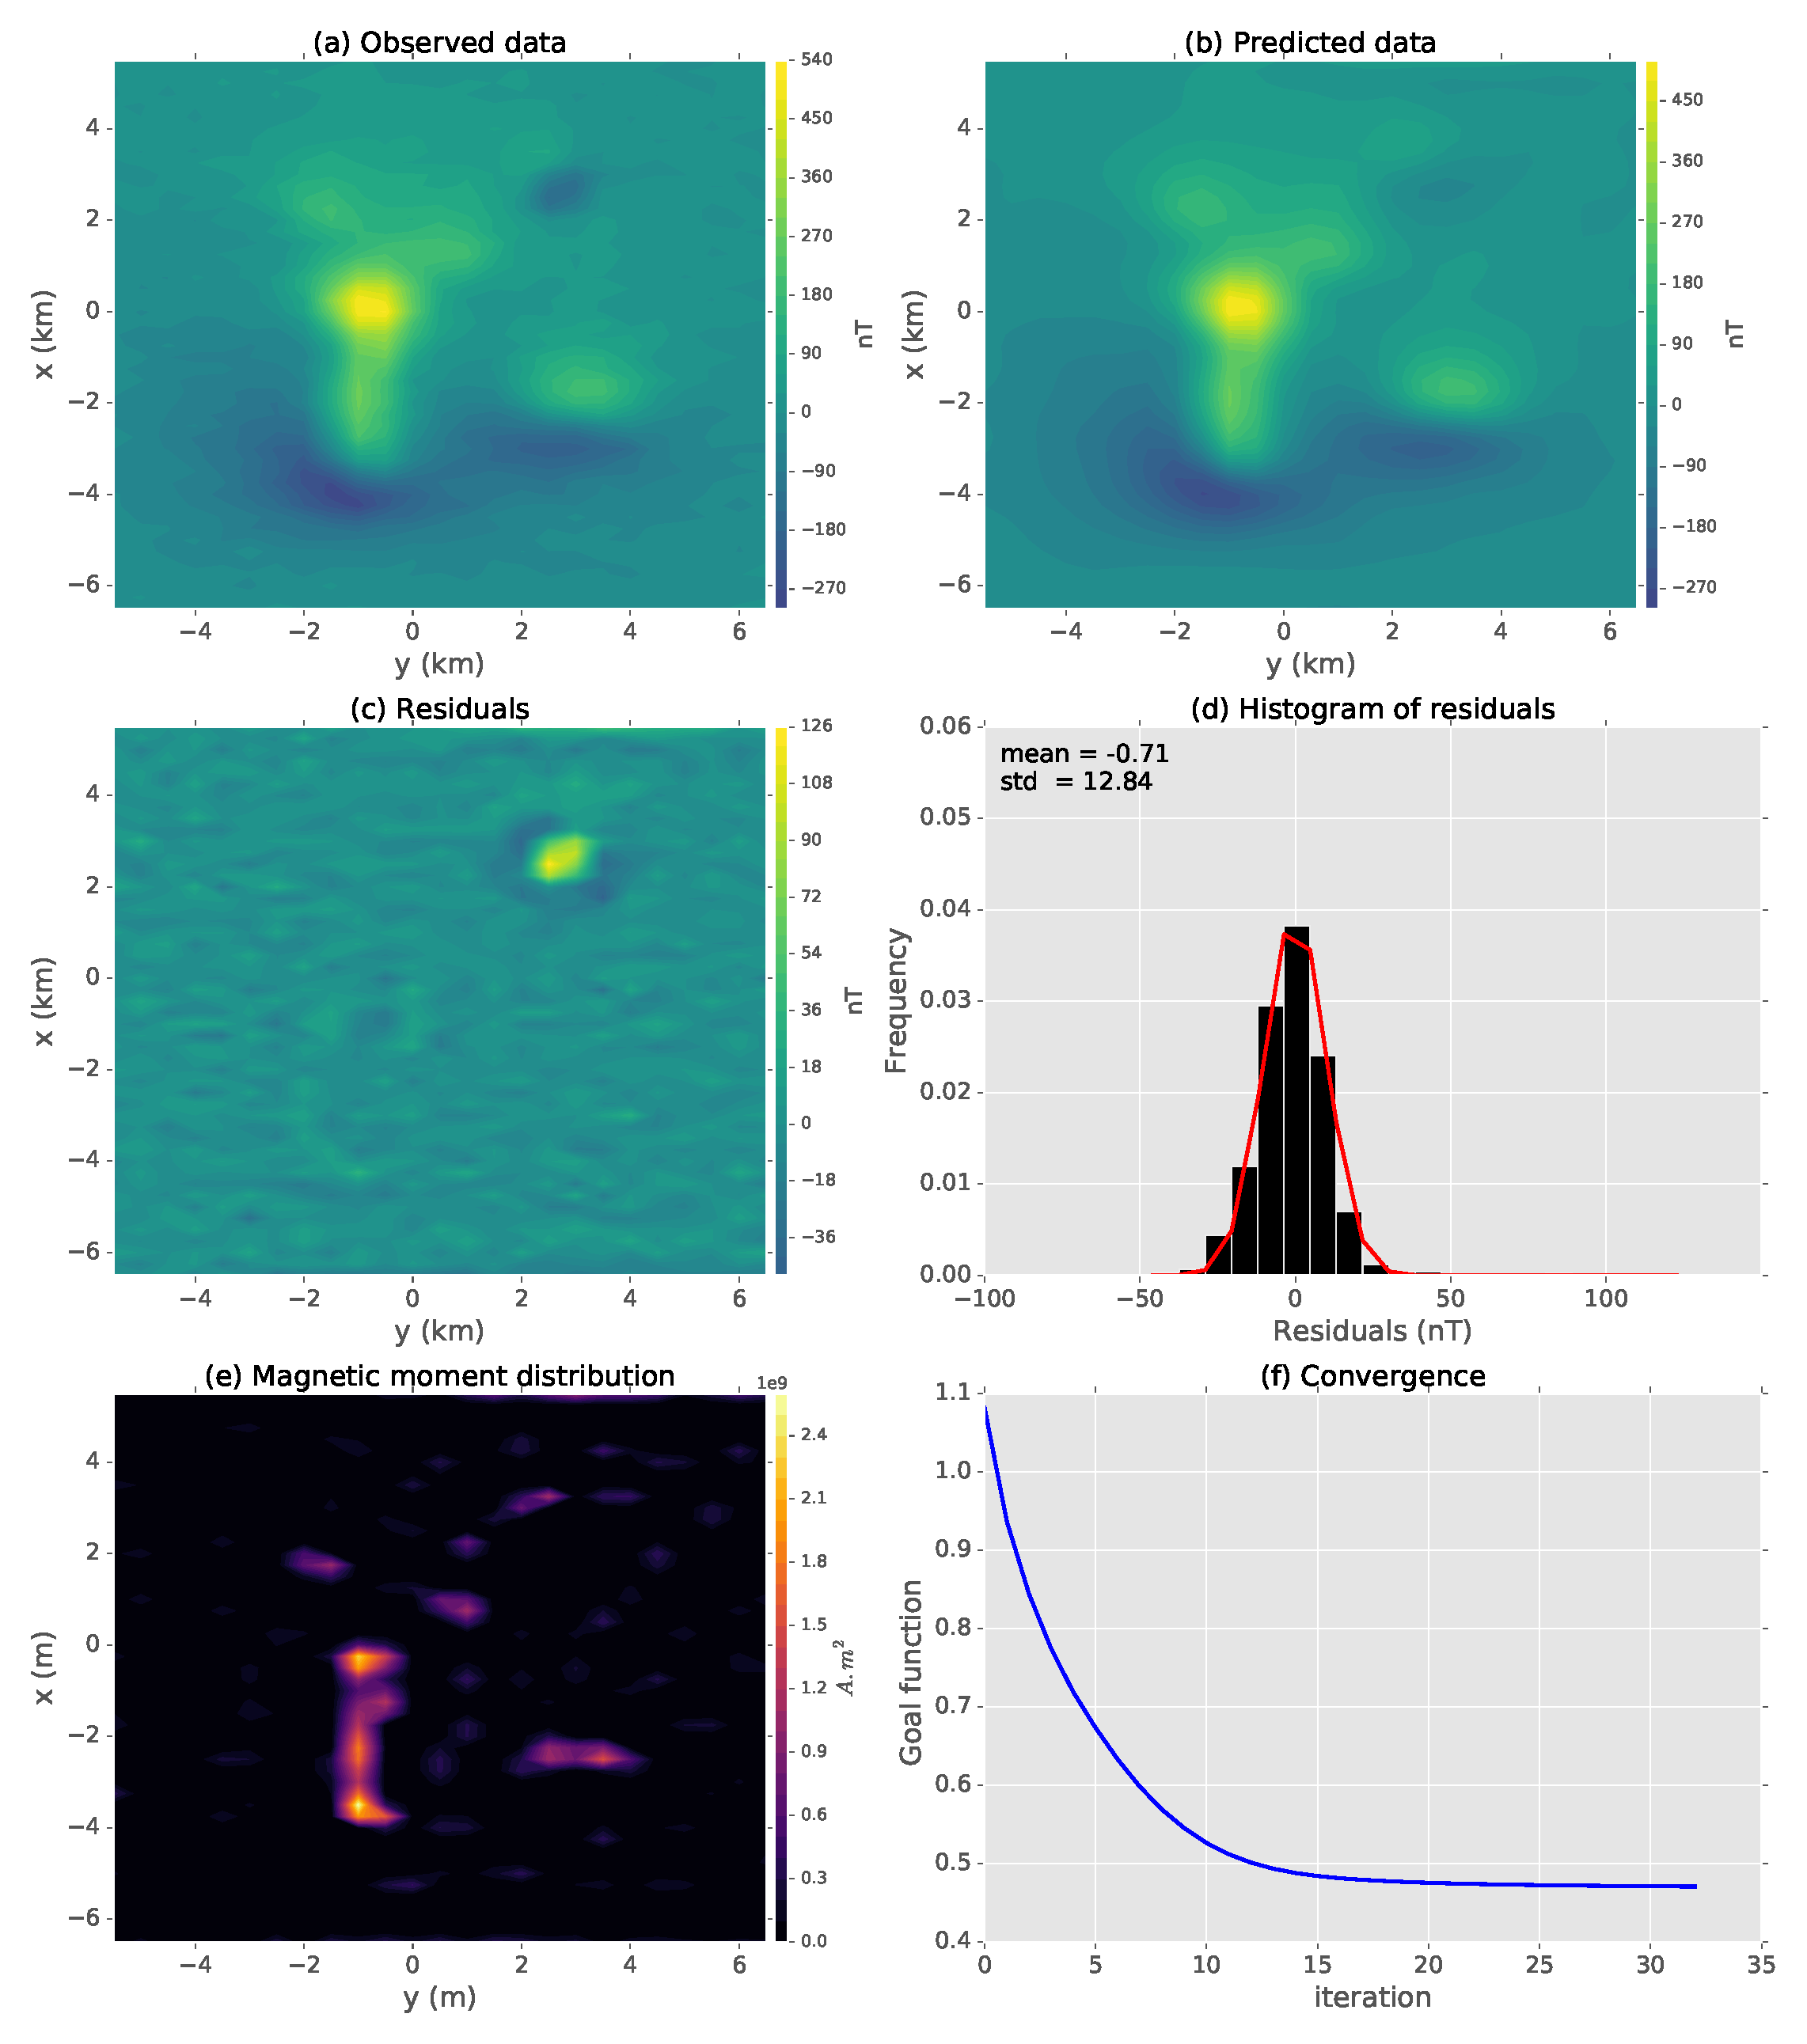
\includegraphics[width=0.85\textwidth]{Fig/unidir_shallow_diff_test/results_compiled_LM_NNLS_magRM.eps}
	\caption{Application to synthetic data with a shallow interfering source with different magnetization direction. (a) Noise-corrupted data. (b) Predicted data produced by equivalent layer. (c) Difference between the data shown in panels (a) and (b). (d) Histogram of residuals. (e) All-positive magnetic moment distribution. (f) Goal function value (equation \ref{eq:positivity_goal_function}a) per iteration showing the convergence.}
	\label{fig:unidir_shallow_diff_test}
\end{figure}

%% Real data application 
\begin{figure}
	\centering
	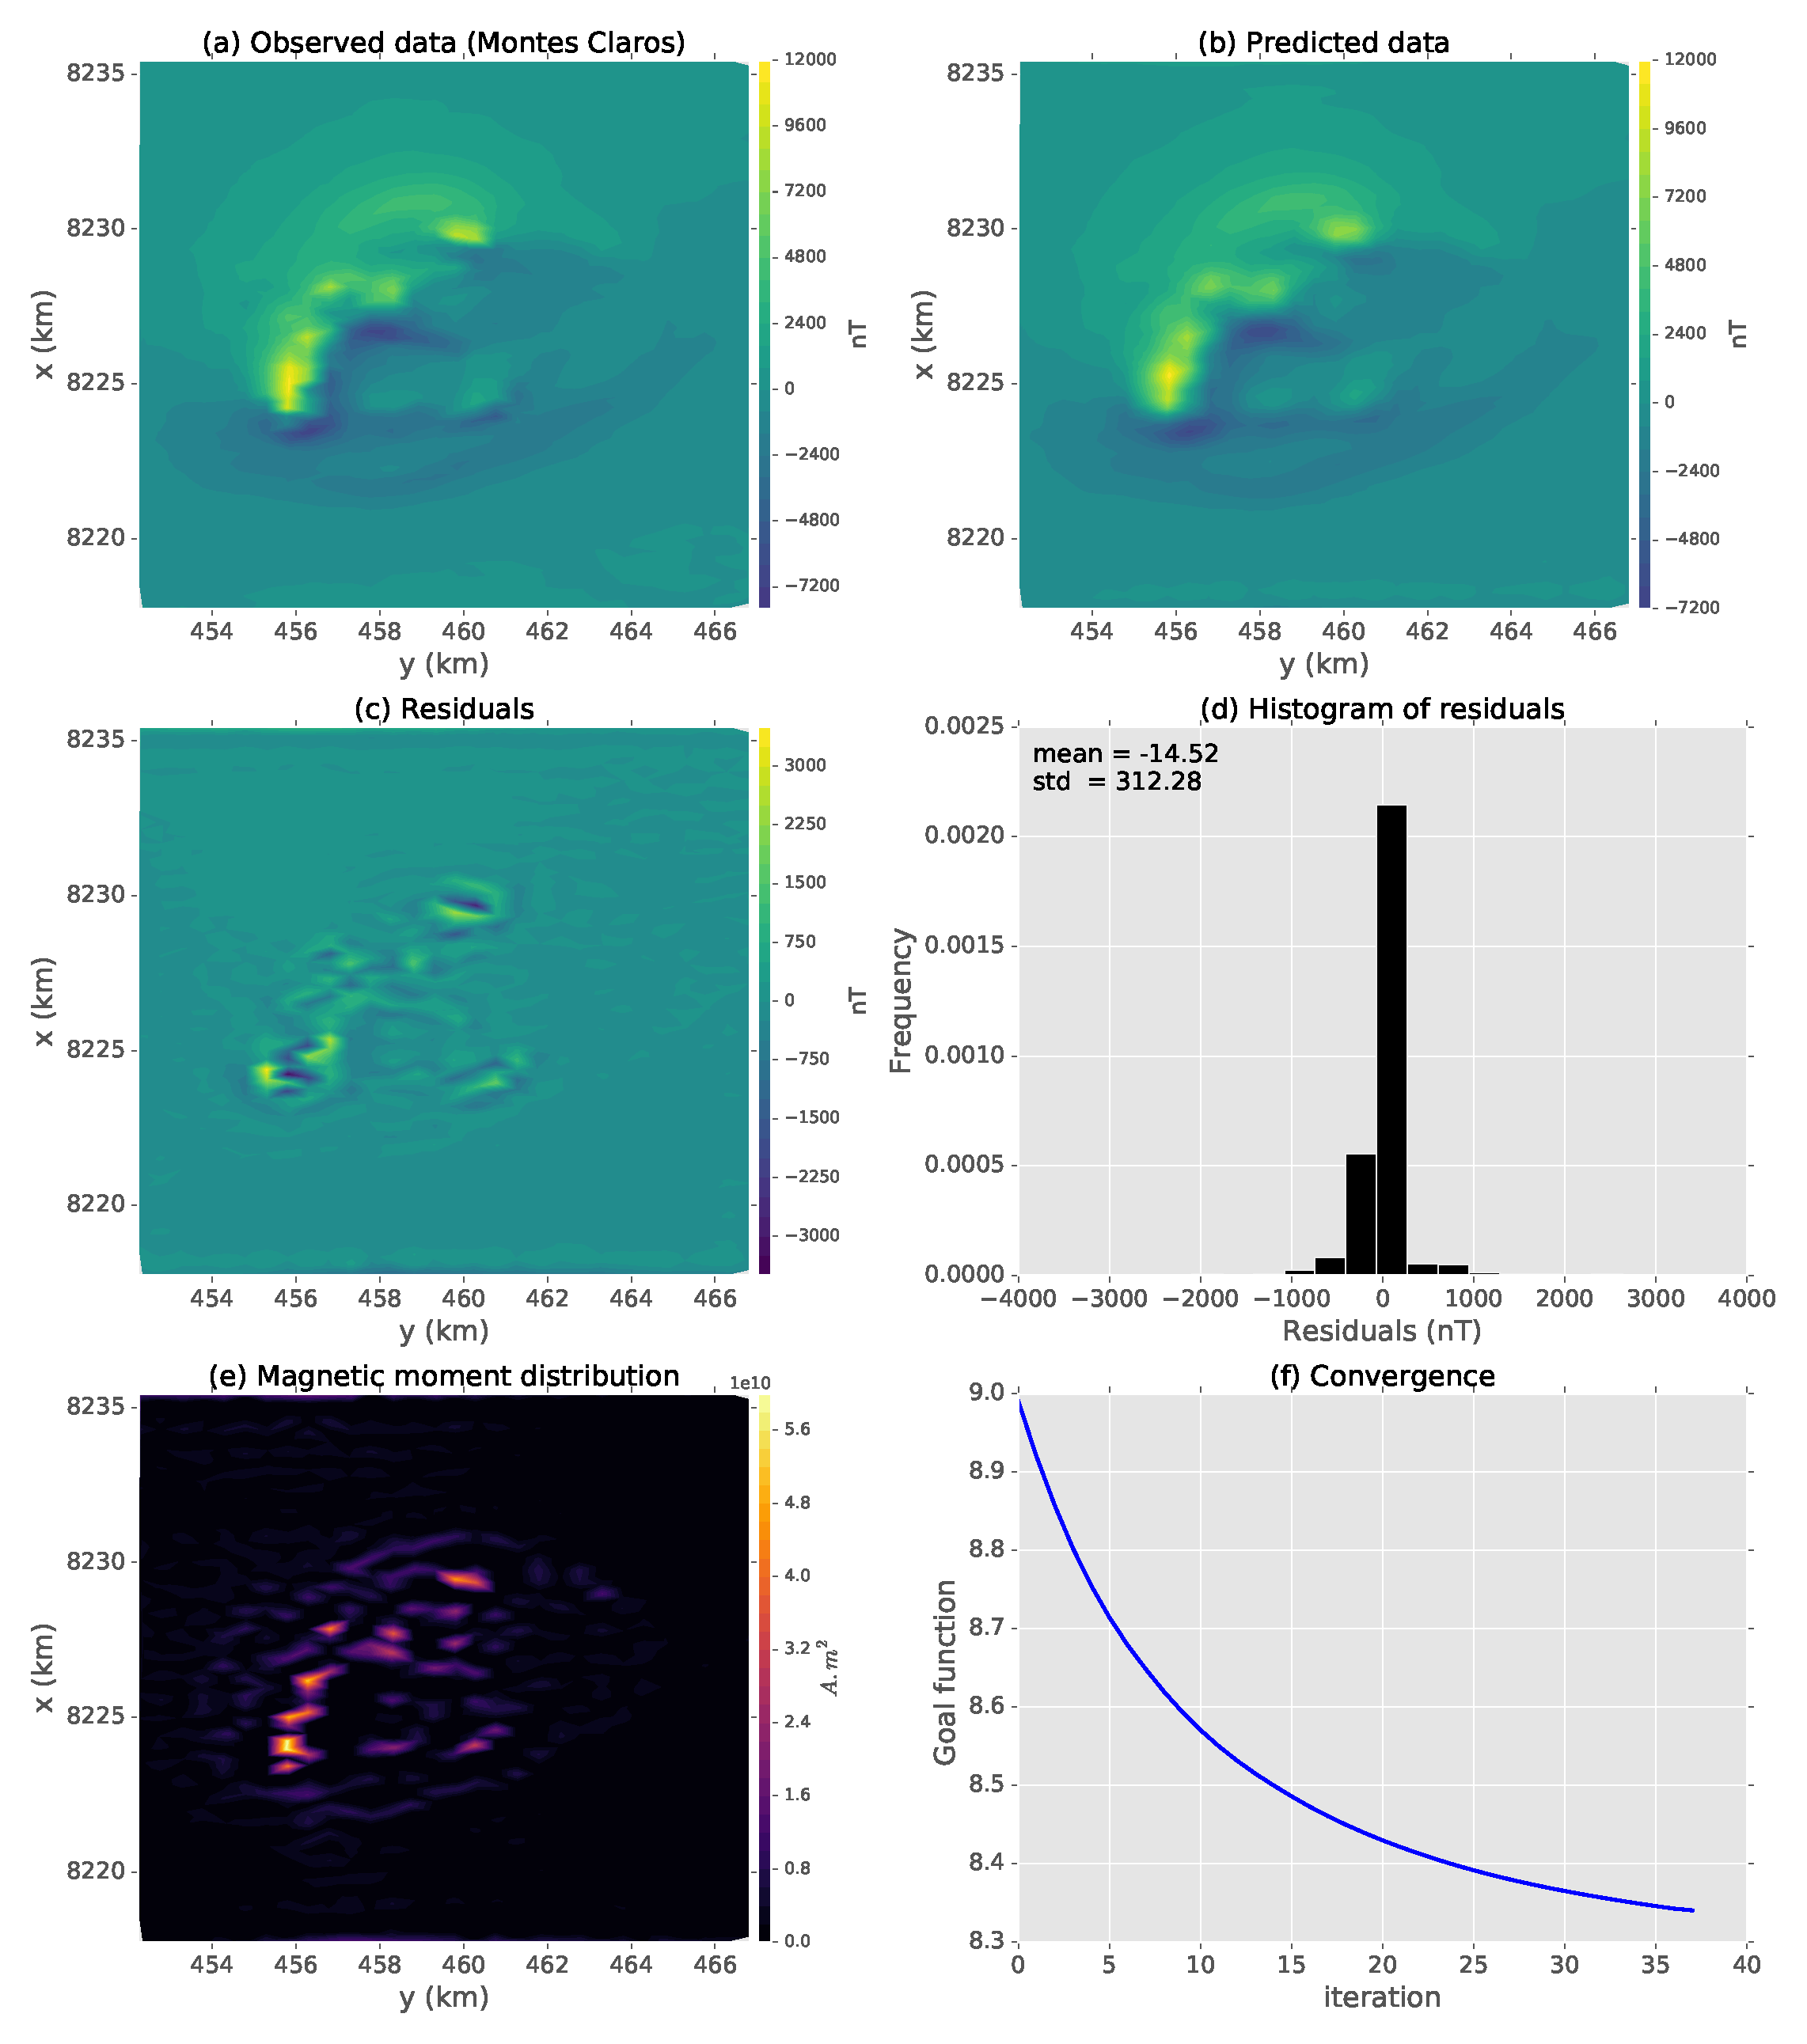
\includegraphics[width=0.85\textwidth]{Fig/field_data_montes_claros/montes_claros_compiled_LM_NNLS_magRM.eps}
	\caption{Application to field data located in complex of Montes Claros. (a) Observation data. (b) Predicted data produced by equivalent layer. (c) Difference between the data shown in panels (a) and (b). (d) Histogram of residuals. (e) All-positive magnetic moment distribution. (f) Goal function value (equation \ref{eq:positivity_goal_function}a) per iteration showing the convergence.}
	\label{fig:mc_data_application}
\end{figure}

\begin{figure}
	\centering
	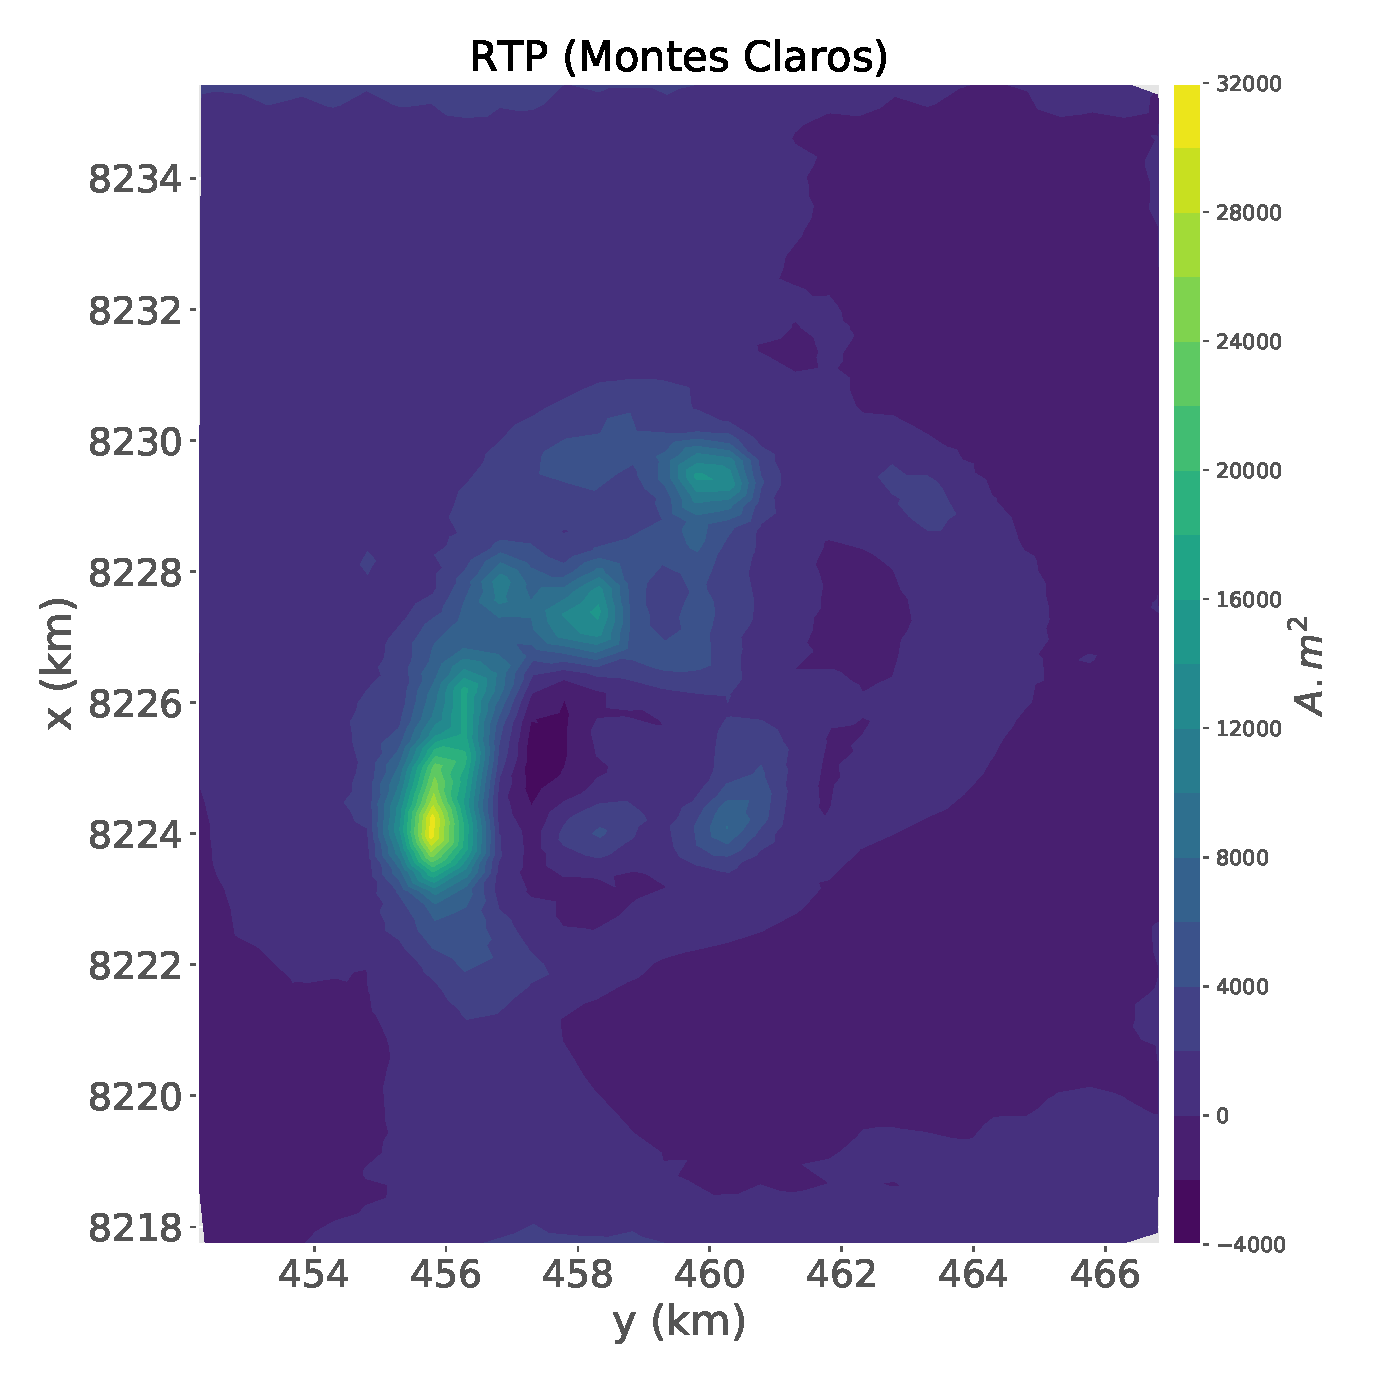
\includegraphics[width=0.75\textwidth]{Fig/field_data_montes_claros/RTP_data_montes_claros.eps}
	\caption{Application to field data located in complex of Montes Claros. RTP anomaly computed by using the estimated magnetization distribution shown in figure \ref{fig:mc_data_application}e.}
	\label{fig:rtp_mc_data}
\end{figure}



\end{document}
